%-----------------------------------------------------------------------
%
\section{Optimization and Autotuning Rules}
\label{autotuning}
%
%-----------------------------------------------------------------------

To provide the possibility to specify any possible combination
between both operation modes, the index (\ref{alpha_pd}), with an
appropriated weight factor $\alpha$ and subjected to the
optimization (\ref{gamma_optimization}), gives the suitable
$\gamma_i$ values that provide the PID tuning according to
(\ref{gammaS_tuning_formulae}).

However, from a more practical point of view is unusual and very
difficult to say for example, that the regulation mode, in a
control system, has the 63\% of the importance (that means the
37\% for the servo). With this respect, we can establish a
categorization in order to make the analysis simpler and also to
help the choice of the weight factor. Therefore, depending on the
operation for the control system, we can identify the following
general cases:

\begin{itemize}

\item Operation only as a servo that means $\alpha=0$.

\item Operation only as a regulator that means $\alpha=1$.

\item Same importance for both system operation modes, servo and
regulation, that is equivalent to $\alpha=0.50$.

\item More importance for the servo than the regulation operation,
that can be expressed by $\alpha=0.25$.

\item More importance for regulator than servo, that can be
indicated as $\alpha=0.75$.

\end{itemize}

This broad classification allows for a qualitative specification
of the control system operation.

Here, the optimization was performed using genetic algorithms
\citep{mitchell1998}, taking problem (\ref{gamma_optimization}) as
the \emph{fitness function}. The implementation was using MATLAB
7.6.0(R2008a)\textregistered{ } for a \emph{population size} of 20
and a maximum number of \emph{generations} of 50.

The optimal solution was found for $\alpha=\{0.25, 0.50, 0.75\}$.
As we said before for $\alpha=\{0, 1\}$, as extreme situations,
the optimal tunings are the related to set-point and
load-disturbance presented previously in Subsection
\ref{tuning-modes}.

It is worth to say that at first the optimization was performed by
considering an enlarged search space for the $\overline{\gamma}$
vector, however, for the rare cases in which the optimal
$\gamma_i$ parameters were outside the interval $[0,1]$, the value
of the objective function was practically the same and, therefore,
it is preferred to constraint the search space in order to provide
a bounded controller's family that is easier to understand as are
presented of an \emph{intermediate} controller.

Tuning relations (\ref{gammaS_tuning_formulae}) allow to select
$\gamma_i$ values on the basis of \emph{trade-off} performance for
both operating modes. However, it would be desirable an automatic
methodology to choose this set of parameters without the need to
run the whole Weighted Performance Degradation analysis.

In order to pursue the previous idea, by repeating the problem
optimization posed in (\ref{gamma_optimization}) for the three
weighting factor and different values of the normalized dead-time
$\tau$, we can find an optimal set for each $\gamma_i$ parameter.
For each one of these groups, it is possible to approximate a
function to determine a general procedure that allows to find the
suitable values for the $\gamma_i$'s, that provide the best
\emph{intermediate} tuning. Results are adjusted to the general
expression as

\be
\gamma_i(\tau)=a+b\tau+c\tau^2 \qquad \tau \in [0.1,1.0] \cup
[1.1,2.0] \label{gammas-eq} \ee

\noindent where $a$, $b$ and $c$ are given in Table
\ref{gammas_settings}, according to the weighting factor $\alpha$
and for each $\gamma_i$ and $\tau$ range. Fig. \ref{gamma1fnc}
shows the followed procedure for $\alpha=0.50$ and the $\gamma_1$
case.

\begin{table}[htb!]
\begin{center}
\caption{$\overline{\gamma}_{\alpha}$ Settings for Autotuning}
\label{gammas_settings}
\begin{tabular}{cc|ccc|ccc}
\cline{2-8} & \textbf{$\tau$ range} &
\multicolumn{3}{c|}{\textbf{0.1 - 1.0}} &
\multicolumn{3}{c}{\textbf{1.1 - 2.0}} \\ \cline{2-8} & constant &
a & b & c & a & b & c \\ \hline
              & \multicolumn{1}{c|}{$\gamma_1$} &0.082 & 0.074 &0.138 &0.021 & 0.040 &-0.006 \\
$\alpha=0.25$ & \multicolumn{1}{c|}{$\gamma_2$} &0.896 &-1.238 &0.854 &0.097 &-0.723 & 0.173 \\
              & \multicolumn{1}{c|}{$\gamma_3$} &0.332 &-0.592 &0.508 &0.323 &-0.183 & 0.033 \\
\hline
              & \multicolumn{1}{c|}{$\gamma_1$} &0.093 & 0.547 &-0.106 & 1.162 &-1.258 & 0.406 \\
$\alpha=0.50$ & \multicolumn{1}{c|}{$\gamma_2$} &0.920 &-0.540 & 0.206 & 2.222 &-2.184 & 0.639 \\
              & \multicolumn{1}{c|}{$\gamma_3$} &0.831 &-1.197 & 0.548 &-0.436 & 0.941 &-0.334 \\
\hline
              & \multicolumn{1}{c|}{$\gamma_1$} &0.108 & 0.566 & 0.067 & 2.197 &-2.529 & 0.774 \\
$\alpha=0.75$ & \multicolumn{1}{c|}{$\gamma_2$} &0.869 &-0.271 & 0.129 & 1.312 &-1.021 & 0.296 \\
              & \multicolumn{1}{c|}{$\gamma_3$} &0.211 & 0.701 &-0.683 &-0.987 & 1.791 &-0.579 \\
\hline
\end{tabular}
\end{center}
\end{table}

\begin{figure}[htb!]
    \begin{center}
        %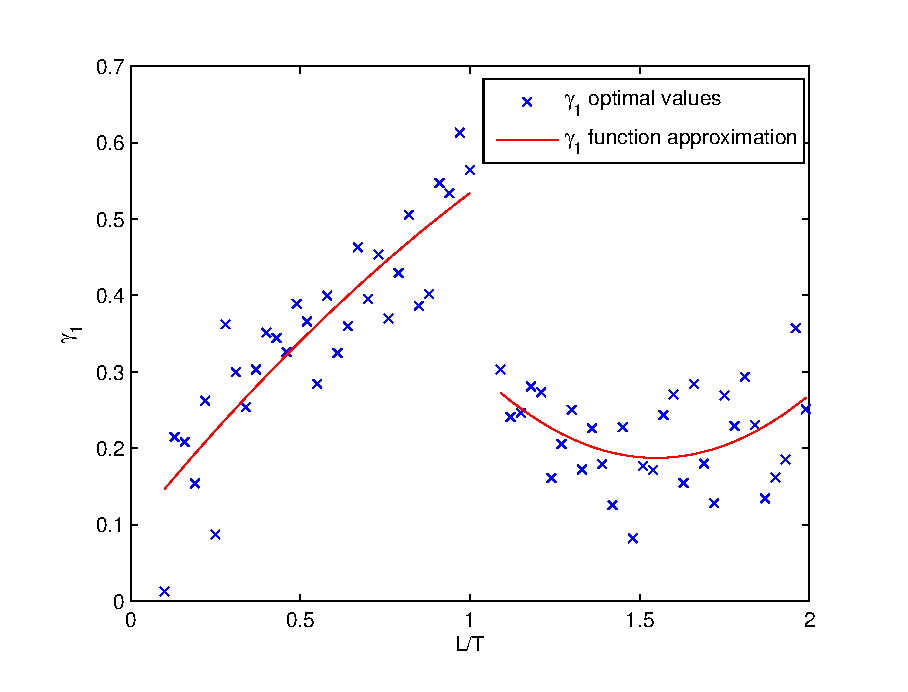
\includegraphics[scale=0.8]{gamma1function.eps}
        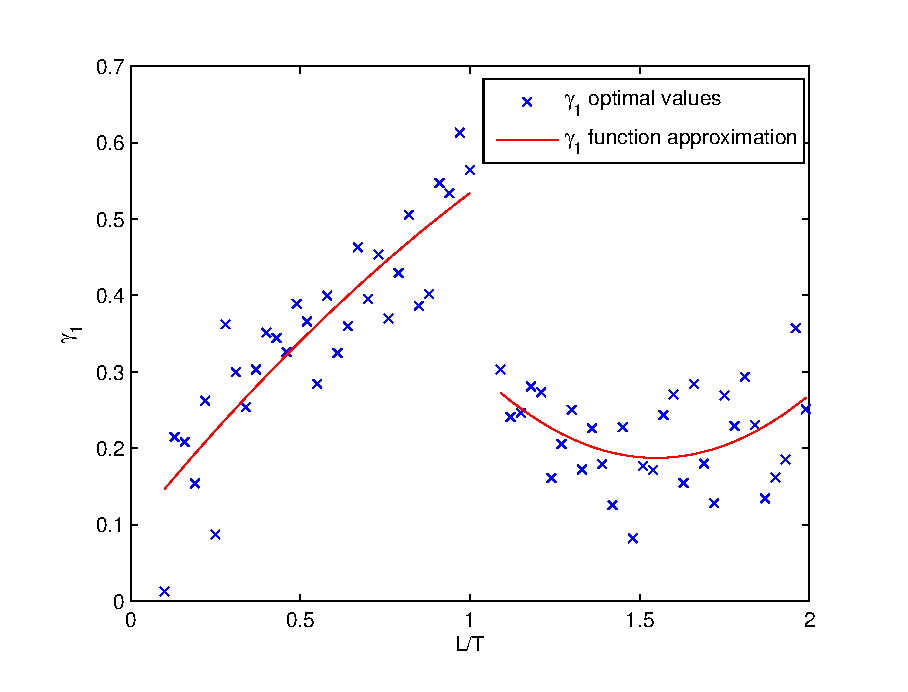
\includegraphics[width=0.8\linewidth]{gamma1function.eps}
        \caption{Optimal set for $\gamma_1$ parameter and the corresponding approximated function for $\alpha=0.50$}
        \label{gamma1fnc}
    \end{center}
\end{figure}

Equation (\ref{gammas-eq}) for each $\gamma_i$ along with the
settings (\ref{gammaS_tuning_formulae}) provide what we call here
$\overline{\gamma}_{\alpha}-autotuning$ for weighted
servo/regulation operation, that is the main contribution of this
paper.
